\documentclass[tikz,border=10pt]{standalone}
\usepackage{helvet}
\renewcommand{\familydefault}{\sfdefault}
\usepackage{amsmath}
\usepackage{tikz}
\usetikzlibrary{calc, positioning, fit, patterns, decorations.pathreplacing, shapes.geometric, arrows.meta}

\definecolor{emeraldpine}{HTML}{1A4D3E}
\definecolor{harvardcrimson}{HTML}{A51C30}
\definecolor{ethdarkblue}{HTML}{1F407A}
\definecolor{ethpetrol}{HTML}{007A87}
\definecolor{ethbronze}{HTML}{B87333}
\definecolor{ethpurple}{HTML}{5B4B8A}
\definecolor{ink}{HTML}{1A202C}
\definecolor{softink}{HTML}{4A5568}
\definecolor{paleink}{HTML}{A0AEC0}
\definecolor{cardbg}{HTML}{F8FAFC}
\definecolor{shadecolor}{HTML}{F4F6F9}

\begin{document}
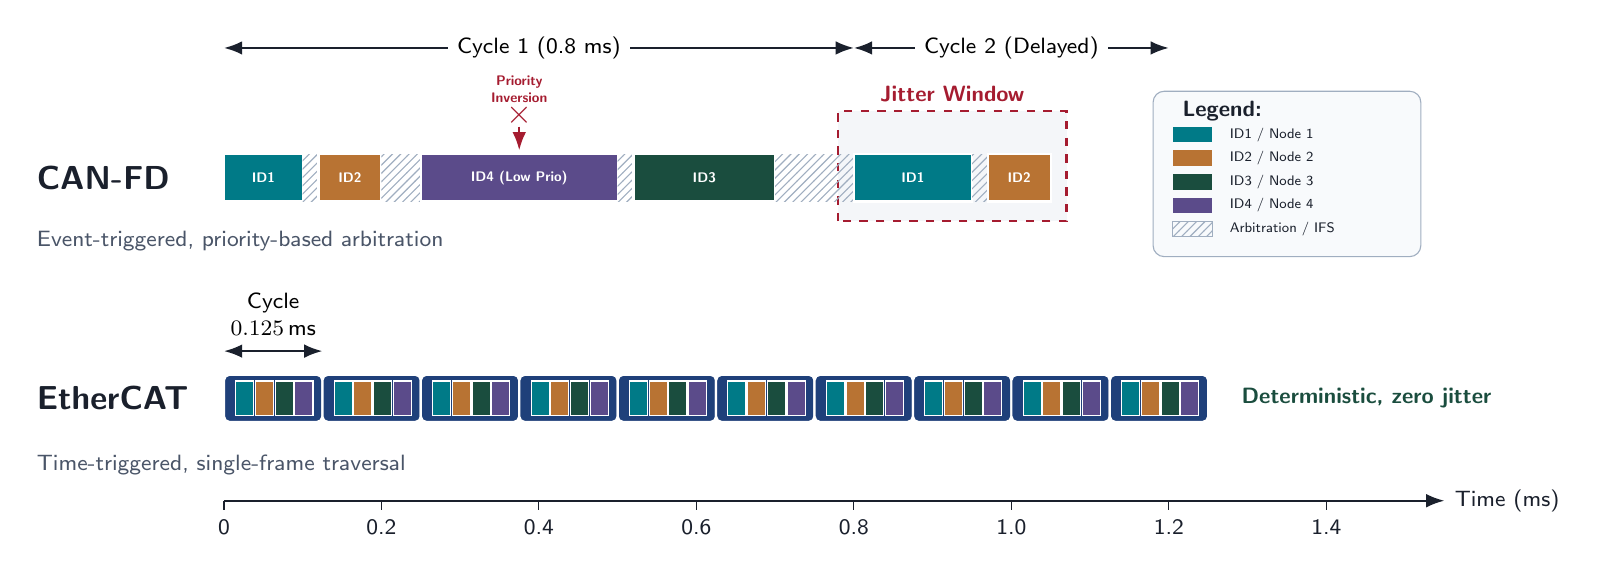
\begin{tikzpicture}[
    x=10cm, y=1cm,
    font=\sffamily,
    frame/.style={draw=white, thick, text=white, align=center, minimum height=0.6cm},
    axis/.style={-Latex, draw=ink, thick},
    tick/.style={draw=ink, thin}
]

    % X-axis
    \draw[axis] (0, 0) -- (1.55, 0) node[right, text=ink, font=\footnotesize] {Time (ms)};
    \foreach \x in {0, 0.2, 0.4, 0.6, 0.8, 1.0, 1.2, 1.4} {
        \draw[tick] (\x, 0) -- (\x, -0.12) node[below, text=ink, font=\footnotesize] {\x};
    }

    % EtherCAT Lane
    \node[anchor=west, text=ink, font=\bfseries\large] at (-0.25, 1.3) {EtherCAT};
    \node[anchor=west, text=softink, font=\footnotesize] at (-0.25, 0.45) {Time-triggered, single-frame traversal};
    
    % Cycles 1 to 10
    \foreach \c in {0, 1, 2, 3, 4, 5, 6, 7, 8, 9} {
        \draw[fill=ethdarkblue, rounded corners=2pt, draw=white, thick] ({\c * 0.125}, 1.0) rectangle ({\c * 0.125 + 0.125}, 1.6);
        \draw[fill=ethpetrol, draw=white] ({\c * 0.125 + 0.015}, 1.08) rectangle ({\c * 0.125 + 0.038}, 1.52);
        \draw[fill=ethbronze, draw=white] ({\c * 0.125 + 0.040}, 1.08) rectangle ({\c * 0.125 + 0.063}, 1.52);
        \draw[fill=emeraldpine, draw=white] ({\c * 0.125 + 0.065}, 1.08) rectangle ({\c * 0.125 + 0.088}, 1.52);
        \draw[fill=ethpurple, draw=white] ({\c * 0.125 + 0.090}, 1.08) rectangle ({\c * 0.125 + 0.113}, 1.52);
    }
    
    \draw[Latex-Latex, draw=ink, thick] (0, 1.9) -- (0.125, 1.9) node[midway, above=2pt, font=\footnotesize, align=center] {Cycle\\$0.125\,\text{ms}$};
    
    \node[text=emeraldpine, font=\footnotesize\bfseries, anchor=west] at (1.28, 1.3) {Deterministic, zero jitter};

    % CAN-FD Lane
    \node[anchor=west, text=ink, font=\bfseries\large] at (-0.25, 4.1) {CAN-FD};
    \node[anchor=west, text=softink, font=\footnotesize] at (-0.25, 3.3) {Event-triggered, priority-based arbitration};
    
    % Jitter Window Background
    \draw[fill=shadecolor, draw=harvardcrimson, dashed, thick] (0.78, 3.55) rectangle (1.07, 4.95);
    \node[text=harvardcrimson, font=\footnotesize\bfseries, anchor=south] at (0.925, 4.95) {Jitter Window};
    
    % CAN-FD Frames
    \draw[fill=ethpetrol, frame] (0, 3.8) rectangle (0.1, 4.4) node[midway, font=\tiny\bfseries] {ID1};
    \draw[pattern=north east lines, pattern color=paleink, draw=none] (0.1, 3.8) rectangle (0.12, 4.4);
    
    \draw[fill=ethbronze, frame] (0.12, 3.8) rectangle (0.2, 4.4) node[midway, font=\tiny\bfseries] {ID2};
    \draw[pattern=north east lines, pattern color=paleink, draw=none] (0.2, 3.8) rectangle (0.25, 4.4);

    \draw[fill=ethpurple, frame] (0.25, 3.8) rectangle (0.5, 4.4) node[midway, font=\tiny\bfseries] {ID4 (Low Prio)};
    \node[text=harvardcrimson, font=\large\bfseries] at (0.375, 4.9) {$\times$};
    \node[text=harvardcrimson, font=\tiny\bfseries, align=center] at (0.375, 5.23) {Priority\\Inversion};
    \draw[-Latex, draw=harvardcrimson, thick] (0.375, 4.75) -- (0.375, 4.45);
    
    \draw[pattern=north east lines, pattern color=paleink, draw=none] (0.5, 3.8) rectangle (0.52, 4.4);
    \draw[fill=emeraldpine, frame] (0.52, 3.8) rectangle (0.7, 4.4) node[midway, font=\tiny\bfseries] {ID3};
    \draw[pattern=north east lines, pattern color=paleink, draw=none] (0.7, 3.8) rectangle (0.8, 4.4);
    
    \draw[fill=ethpetrol, frame] (0.8, 3.8) rectangle (0.95, 4.4) node[midway, font=\tiny\bfseries] {ID1};
    \draw[pattern=north east lines, pattern color=paleink, draw=none] (0.95, 3.8) rectangle (0.97, 4.4);
    \draw[fill=ethbronze, frame] (0.97, 3.8) rectangle (1.05, 4.4) node[midway, font=\tiny\bfseries] {ID2};
    
    \draw[Latex-Latex, draw=ink, thick] (0, 5.75) -- (0.8, 5.75) node[midway, fill=white, font=\footnotesize] {Cycle 1 (0.8 ms)};
    \draw[Latex-Latex, draw=ink, thick] (0.8, 5.75) -- (1.2, 5.75) node[midway, fill=white, font=\footnotesize] {Cycle 2 (Delayed)};

    % Legend
    \begin{scope}[shift={(1.18, 3.1)}]
        \draw[fill=cardbg, draw=paleink, rounded corners=4pt] (0, 0) rectangle (0.34, 2.1);
        \node[font=\footnotesize\bfseries, anchor=west, text=ink] at (0.025, 1.85) {Legend:};
        
        \draw[fill=ethpetrol, draw=none] (0.025, 1.45) rectangle (0.075, 1.65);
        \node[anchor=west, font=\tiny, text=ink] at (0.085, 1.55) {ID1 / Node 1};
        
        \draw[fill=ethbronze, draw=none] (0.025, 1.15) rectangle (0.075, 1.35);
        \node[anchor=west, font=\tiny, text=ink] at (0.085, 1.25) {ID2 / Node 2};
        
        \draw[fill=emeraldpine, draw=none] (0.025, 0.85) rectangle (0.075, 1.05);
        \node[anchor=west, font=\tiny, text=ink] at (0.085, 0.95) {ID3 / Node 3};
        
        \draw[fill=ethpurple, draw=none] (0.025, 0.55) rectangle (0.075, 0.75);
        \node[anchor=west, font=\tiny, text=ink] at (0.085, 0.65) {ID4 / Node 4};
        
        \draw[pattern=north east lines, pattern color=paleink, draw=paleink] (0.025, 0.25) rectangle (0.075, 0.45);
        \node[anchor=west, font=\tiny, text=ink] at (0.085, 0.35) {Arbitration / IFS};
    \end{scope}

\end{tikzpicture}
\end{document}
